% !TEX TS-program = lualatex
% !TEX encoding = UTF-8 Unicode

\documentclass{report}
\usepackage[utf8]{inputenc}
% 页眉
\usepackage{fancyhdr}
% 为中文 / 日语提供注音
\usepackage{luatexja-ruby}
% 代码高亮
\usepackage{minted}
% 页面布局
\usepackage[
  papersize={8.5in,11in},
  a4paper,
  bindingoffset=0.2in,
  left=1.2in,
  right=1.2in,
  top=1in,
  bottom=1in,
  footskip=.25in,
  headheight=14pt,
]{geometry}
% 预定义颜色
\usepackage[dvipsnames]{xcolor}
% 超链接
\usepackage[
  colorlinks,
  linkcolor = BrickRed,
  citecolor = Green,
  filecolor = Mulberry,
  urlcolor  = NavyBlue,
  menucolor = BrickRed,
  runcolor  = Mulberry,
]{hyperref}
% 参考文献
\usepackage[
  backend  = biber,
  style    = caspervector,
  seconds,
  utf8,
  backref,
]{biblatex}
% 页脚
\usepackage[
  perpage,
  hang,
  flushmargin,
]{footmisc}
% 多行页脚
\usepackage{footnotebackref}
% 字体
\usepackage{pifont}
% 图像
\usepackage{graphicx}
% 扫描本地字体
\usepackage{fontspec}
% 控制章节标题格式
\usepackage{sectsty}
% 详见 https://tex.stackexchange.com/questions/664/why-should-i-use-usepackaget1fontenc
\usepackage[T1]{fontenc}
% Letter Spacing
% 详见 https://tex.stackexchange.com/questions/522106/is-there-a-way-to-get-wider-spacing-between-the-letters
\usepackage{soul} 
% 控制章节标题格式
\usepackage[explicit]{titlesec}
% 控制 TOC 目录格式
\usepackage{titletoc}
% 控制列表格式
\usepackage[shortlabels]{enumitem}
% 彩色框 - 本模板用于定义定理,定义,例子的框图样式
% 详见 https://tex.stackexchange.com/questions/562753/how-to-make-a-colour-box-in-these-3-different-ways
\usepackage{tcolorbox}
% Pst-node 节点绘图
\usepackage{pst-node}
% Tikz 绘图
\usepackage{tikz}
% Tikz 交换图绘图
\usepackage{tikz-cd}
% pgf 函数绘图
\usepackage{pgfplots}
\usetikzlibrary{positioning}
\usetikzlibrary{arrows}

% RSFS 字体
% 详解 https://tug.org/FontCatalogue/ralphsmithsformalscript/
\usepackage{mathrsfs}
% 数学
\usepackage{amssymb}
\usepackage{mathtools}
\usepackage{amsthm}
\usepackage{amsmath}
% 划线抵消删除符号
\usepackage{cancel}

% 浮动体,提供 [H] `PUT IT HERE` 选项
\usepackage{float}
% 提供更细粒度的浮动体 Caption 控制
\usepackage{caption}
% 提供并排浮动体的子 Caption 控制(左右排列的图片使用不同的 Caption)
\usepackage{subcaption}
% 提供多列的文章排版
\usepackage{multicol}
% 提供更细粒度的表格宽度控制
\usepackage{tabularx}
% 希腊字母
\usepackage{upgreek}
% 修改字体 / 数学字符的大小
\usepackage{relsize}

% 注释块
\usepackage{verbatim}

% 用于生成测试文本, 可以删除
\usepackage{blindtext}

% 图像资源路径
\graphicspath{{images/}}

% 重定义粗体,以使其字体统一
\renewcommand{\emph}[1]{\textbf{#1}}

% 参考文献
\addbibresource{ref.bib}

% 代码块
\renewcommand{\theFancyVerbLine}{%
  \ttfamily {%
    \oldstylenums{\arabic{FancyVerbLine}}
  }
}
\setminted{
  mathescape,
  linenos,
  breaklines,
  breakanywhere,
  autogobble,
  numbersep=5pt,
  baselinestretch=1.2,
  frame    = lines,
  framesep = 2mm,
}

% 字体
\setmainfont{New York Small Regular}[
  ItalicFont = New York Small Regular Italic
]
\setsansfont{SF Pro Text}[
  ItalicFont = New York Small Regular Italic
]

\newcommand{\emoji}[1]{
  {\setmainfont{Apple Color Emoji}[Renderer=Harfbuzz]{#1}}
}

\setmonofont[
  ItalicFont     = JetBrains Mono Italic,
  BoldFont       = JetBrains Mono Bold,
  BoldItalicFont = JetBrains Mono Bold Italic,
  Contextuals    = Alternate,
]{JetBrains Mono}

\newfontfamily\lmmono{Latin Modern Mono}
\newfontfamily\bsans{SF Pro Text Bold}
\newfontfamily\displaysans{SF Pro Display}

% 设置所有章节标题字体为非衬线字体
\allsectionsfont{\displaysans}

\sodef\chapterso{}{.5em}{2em}{2em}

% 设置章节标题样式
\titleformat{\chapter}[display]
{\bfseries} %format
{\textsf{\textbf{\large\chapterso{\MakeUppercase\chaptertitlename}\hspace{1.1em}\thechapter}}} %label
{1.5em} %sep 
{\displaysans{\textbf{\huge#1}}\bfseries} %before-code

\titlespacing*{\chapter}{0pt}{-30pt}{40pt}

% 设置 TOC 样式
\titlecontents{chapter}
[1.5em]
{\sf}
{\bsans Chapter \thecontentslabel. }
{\huge}
{\mdseries\titlerule*[0.75em]{.}\bfseries \thecontentspage} 
[\addvspace{.5pc}]

\titlecontents{section}
[2.5em]
{\sf}
{\thecontentslabel. }
{\huge}
{\mdseries\titlerule*[0.75em]{.}\bfseries \thecontentspage} 
[\addvspace{.5pc}]

\titlecontents{subsection}
[3.5em]
{\sf}
{\thecontentslabel. }
{\huge}
{\mdseries\titlerule*[0.75em]{.}\bfseries \thecontentspage} 
[\addvspace{.5pc}]

\titlecontents{subsubsection}
[3.5em]
{\sf}
{\thecontentslabel. }
{\huge}
{\mdseries\titlerule*[0.75em]{.}\bfseries \thecontentspage} 
[\addvspace{.5pc}]

% 链接样式
\urlstyle{same}
\let\oldurl\url
\renewcommand{\url}[1]{%
{\lmmono\oldurl{#1}}
}

% 彩色定理 / 例子 / 定义环境
\definecolor{theorembg}{HTML}{F2F2F9}
\definecolor{theoremfr}{HTML}{00007B}
\definecolor{examplebg}{HTML}{F8E5D5}
\definecolor{examplefr}{HTML}{FA893F}
\definecolor{exampleti}{HTML}{2A7F7F}
\definecolor{definitbg}{HTML}{DEFFD4}
\definecolor{definitfr}{HTML}{60AD49}
\theoremstyle{definition}
\newtheorem{definition}{Definition}
\newtheorem{example}{Example}
\newtheorem{theorem}{Theorem}
\newtheorem{corollary}{Corollary}[theorem]
\newtheorem{lemma}[theorem]{Lemma}
\newtheorem*{remark}{Remark}
\newtheorem{exercise}{Exercise}
\newtheorem{problem}{Problem}
\newtheorem{proposition}{Proposition}
\newtheorem{question}{Question}
\newtheorem{conjecture}{Conjecture}
\newtheorem{assumption}{Assumption}
\newtheorem{notation}{Notation}
\newtheorem{claim}{Claim}
\newtheorem{observation}{Observation}
\newtheorem{fact}{Fact}
\newtheorem{solution}{Solution}
\newtheorem{convention}{Convention}


\tcbuselibrary{theorems,skins,hooks}

\newtcbtheorem[number within=section]{Theorem}{Theorem}
{%
   enhanced
  ,colback = theorembg
  ,frame hidden
  ,boxrule = 0sp
  ,borderline west = {2pt}{0pt}{theoremfr}
  ,sharp corners
  ,detach title
  ,before upper = \tcbtitle\par\smallskip
  ,coltitle = theoremfr
  ,fonttitle = \bfseries\sffamily
  ,description font = \mdseries
  ,terminator sign none
  ,separator sign none
}
{th}

\newtcbtheorem[number within=section]{Example}{Example}
{%
   enhanced
  ,colback = examplebg
  ,frame hidden
  ,boxrule = 0sp
  ,borderline west = {2pt}{0pt}{examplefr}
  ,sharp corners
  ,detach title
  ,before upper = \tcbtitle\par\smallskip
  ,coltitle = examplefr
  ,fonttitle = \bfseries\sffamily
  ,description font = \mdseries
  ,terminator sign none
  ,separator sign none
}
{ex}


\newtcbtheorem[number within=section]{Definition}{Definition}
{%
   enhanced
  ,colback = definitbg
  ,frame hidden
  ,boxrule = 0sp
  ,borderline west = {2pt}{0pt}{definitfr}
  ,sharp corners
  ,detach title
  ,before upper = \tcbtitle\par\smallskip
  ,coltitle = definitfr
  ,fonttitle = \bfseries\sffamily
  ,description font = \mdseries
  ,terminator sign none
  ,separator sign none
}
{def}

%% Backref
\makeatletter
\LetLtxMacro{\BHFN@Old@footnotemark}{\@footnotemark}

\renewcommand*{\@footnotemark}{%
    \refstepcounter{BackrefHyperFootnoteCounter}%
    \xdef\BackrefFootnoteTag{bhfn:\theBackrefHyperFootnoteCounter}%
    \label{\BackrefFootnoteTag}%
    \BHFN@Old@footnotemark
}
\makeatother


% 页眉
\fancyhf{}
\renewcommand{\headrulewidth}{0pt}
% \renewcommand\headrule{\makebox[\textwidth][r]{\rule{0.4\headwidth}{\headrulewidth}}}
\renewcommand{\sectionmark}[1]{\markright{#1}}
\rhead{\sf{\rightmark} \hspace{.8em} \bsans{\thepage}}
\pagestyle{fancy}


% 页脚
\fancyfoot[C]{\thepage}

\author{Colerar}
\date{\today}
\title{Lua\LaTeX General Template}

\begin{document}

% 标题
\maketitle

% 目录
{
  \hypersetup{linkcolor=black}
  \tableofcontents
}

% --- 预定义快捷方式 ---

\newcommand{\ra}{\rightarrow}
\newcommand{\la}{\leftarrow}
\newcommand{\suchthat}{\textnormal{ such that }}
\newcommand{\for}{\textnormal{ for }}
\newcommand{\where}{\textnormal{ where }}
\newcommand{\by}{\textnormal{ by }}
\newcommand{\and}{\textnormal{ and }}

\newcommand{\R}{\mathbb{R}}
\newcommand{\Z}{\mathbb{Z}}
\newcommand{\N}{\mathbb{N}}
\newcommand{\Q}{\mathbb{Q}}
\newcommand{\M}{\mathbb{M}}
\newcommand{\C}{\mathbb{C}}
\newcommand{\F}{\mathbb{F}}

\renewcommand{\P}{\mathcal{P}}
\newcommand{\T}{\mathcal{T}}
\newcommand{\D}{\mathcal{D}}
\newcommand{\U}{\mathcal{U}}
\newcommand{\V}{\mathcal{V}}
\newcommand{\card}{\textnormal{card}}

\newcommand{\Mmn}{\M_{m,n}}
\newcommand{\FF}[2]{\F^{#1 \times #2}}
\newcommand{\RR}[2]{\R^{#1 \times #2}}
\newcommand{\CC}[2]{\C^{#1 \times #2}}
\newcommand{\seq}[1]{\{#1_i\}_{i=1}^{\infty}}
\newcommand{\trace}{\operatorname{tr}}
\newcommand{\rsa}{\rightsquigarrow}
\newcommand{\rank}{\operatorname{rank}}
\newcommand{\diag}{\operatorname{diag}}
\newcommand{\spann}[1]{\operatorname{span}(#1)}
\newcommand{\proj}{\operatorname{proj}}
\newcommand{\vol}{\operatorname{vol}}
\newcommand{\cis}{\operatorname{cis}}
\newcommand{\Sym}{\operatorname{Sym}}
% partial qed
\newcommand{\qedp}{\hfill $\square$}

\newcommand{\mat}[1]{\begin{bmatrix} #1 \end{bmatrix}}
\newcommand{\vmat}[1]{\begin{vmatrix} #1 \end{vmatrix}}
\newcommand{\pmat}[1]{\begin{pmatrix} #1 \end{pmatrix}}
\DeclarePairedDelimiter\ceil{\lceil}{\rceil}
\DeclarePairedDelimiter\floor{\lfloor}{\rfloor}

\renewcommand\labelenumi{(\theenumi)}
\renewcommand\qedsymbol{$\blacksquare$}

% --- 正文 ---

\chapter{Lorem Ipsum}


\section{Lorem Ipsum 2}

\emph{\ltjruby{Lorem}{ipsum}} dolor sit amet, \textit{aeque labores expetendis} vim an, eu ius atqui sensibus. Mollis suscipit vivendum sed id. Eos ex fuisset accusam. Quo natum autem at, blandit dissentiet in usu, cum porro aeque probatus ea.

\section{Lorem}

\emph{Lorem} ipsum dolor sit amet, aeque labores expetendis vim an, eu ius atqui sensibus. Mollis suscipit vivendum sed id. Eos ex fuisset accusam. Quo natum autem at, blandit dissentiet in usu, cum porro aeque probatus ea.

Ius tale phaedrum democritum id. Vel ut dico munere doctus, nec ei dicant referrentur. Te sanctus consequat maiestatis ius, autem facete at sed. Has te nobis malorum democritum, vocent alterum pri ne, sit dicit possim no. Noster intellegebat ius at, an diam saepe vis.

Ut eros admodum antiopam his. Iuvaret docendi platonem at usu, cu ornatus accusam conclusionemque ius, id nulla diceret fabellas vim. Ut his essent dignissim, id mei aperiri corpora. Qui ad modus senserit torquatos, no reque adipisci honestatis nec.

Ius cibo latine te, probatus deterruisset mei et, ea est possit semper scaevola. Putent putant ea per, ex ipsum inani graecis cum. Est te duis nobis assentior\footnote{atqui patrioque definiebas} duo id, at modus animal eum. Porro graece reprimique eos in, mea in vulputate constituto. Sit errem postea quaeque ei. Nusquam quaestio eloquentiam vix an, ad probo mandamus persecuti has. Cum oratio delicatissimi ei, veniam homero qualisque sed ea, ius voluptatum definitionem ad.


\newpage
\section{仮名} \label{sec:kana}

\emph{\ltjruby{仮名}{かな}}とは、漢字をもとにして日本で作られた文字のこと。
現在一般には平仮名と片仮名のことを指す。表音文字の一種であり、基本的に1字が1音節を
あらわす音節文字に分類される。漢字に対して\ltjruby{和字}{わじ}ともいう。ただし和字は和製漢字を
意味することもある。

\section{Section}

\subsection{Subsection}
\subsection{Subsection}
\subsubsection{Subsubsection}

\paragraph{Paragraph} This is a paragraph.  Lorem ipsum dolor sit amet, aeque labores expetendis vim an, eu ius atqui sensibus. Mollis suscipit vivendum sed id. Eos ex fuisset accusam. Quo natum autem at, blandit dissentiet in usu, cum porro aeque probatus ea.
\subparagraph{Subparagraph} This is a subparagraph. Lorem ipsum dolor sit amet, aeque labores expetendis vim an, eu ius atqui sensibus. Mollis suscipit vivendum sed id. Eos ex fuisset accusam. Quo natum autem at, blandit dissentiet in usu, cum porro aeque probatus ea.

\newpage
\section{Code Block}

\begin{minted}{haskell}
import Control.Monad.State
fib n = flip evalState (0, 1) $ do
  forM [0..(n - 1)] $ \_ -> do
    (a, b) <- get
    put (b, a + b)
  (a, b) <- get
  return a
\end{minted}

Following code block has been highlighted.

\begin{minted}[
  highlightlines={6-9}
]{kotlin}
suspend fun main(args: Array<String>) {
  when (val result = SorapointaMain().main(args)) {
      is CommandResult.Success -> {
          exitProcess(0)
      }
      is CommandResult.Error -> {
          println(result.userMessage)
          exitProcess(1)
      }
  }
}
\end{minted}


\newpage
\section{Figure}

\autoref{fig:example} from Pexels\textsuperscript{\copyright{}}.

\begin{figure}[htbp]
  \centering
  \includegraphics[scale=0.2]{pexels-1509534.jpg}
  \caption{From Pexels \url{https://www.pexels.com/photo/1509534/}}
  \label{fig:example}
\end{figure}

\begin{figure}[htbp]
\centering
\includegraphics[scale=0.2]{pexels-1509534.jpg}
\includegraphics[scale=0.2]{pexels-1509534.jpg}
\\[\smallskipamount]
\includegraphics[scale=0.2]{pexels-1509534.jpg}
\includegraphics[scale=0.2]{pexels-1509534.jpg}
\caption{Multiple Figures Layout}
\end{figure}


\newpage
\section{Others}

\begin{description}
  \item[Link] \url{https://www.example.com}
  \item[Link with description] \href{https://www.ctan.org}{CTAN}
  \item[Jump Link] \hyperref[sec:kana]{Click here to jump to {仮名}}
  \item[Emoji] \emoji{😶‍🌫️😂👍👪} 
  % \item[References] Lorem ipsum \ldots \autocite{greenwade93}
  \item[Footnote Link\footnotemark] See below
  \footnotetext{\href{https://example.org}{Example}}
  \item[Multi-line text in footnote\footnotemark] See below
  \footnotetext{%
    Multi-line text also can be easily aligned.\\
    Provided by \texttt{footmisc} package.
  }
\end{description}

\section{Your boxes}
An example theorem is shown in theorem~\ref{th:pnt}, and there is
example~\ref{ex:bertrand}.

\begin{Theorem}{Prime Number Theorem (PNT)}{pnt}
  \begin{equation*}
    \pi(x)\sim\frac{x}{\log x}
  \end{equation*}
\end{Theorem}
\begin{Example}{Generalisation of Bertrand's Postulate}{bertrand}
  Let $\varepsilon>0$. Prove that there exist a prime between $n$ and
  $(1+\varepsilon)n$ for all large $n$, in particular there always exist a
  prime between $n$ and $2n$ for $n>1$.
\end{Example}
\begin{Definition}{Ordinary}
  An ordinary differential equation, often abbreviated as an ODE, is a
  differential equation that is in the form of:
  \begin{equation*}
    F(x,y,y',y''\cdots)=0
  \end{equation*}
\end{Definition}

\chapter{TikZ Diagram}

\tikzset{
  box/.style ={
    rectangle, %矩形节点
    rounded corners =5pt, %圆角
    minimum width =50pt, %最小宽度
    minimum height =20pt, %最小高度
    inner sep=5pt, %文字和边框的距离
    draw=blue %边框颜色}
  }
}

\begin{tikzpicture}
  \node[box] (1) at(0,0) {1};
  \node[box] (2) at(4,0) {2};
  \node[box] (3) at(8,0) {3};
  \draw[->] (1)--(2);
  \draw[->] (2)--(3);
  \node at(2,1) {a};
  \node at(6,1) {b};
  \end{tikzpicture}

\begin{tikzpicture}[sibling distance =80pt]
  \node[box] {1}
      child {node[box] {2}}
      child {node[box] {3}
          child {node[box] {4}}
          child {node[box] {5}}
          child {node[box] {6}}
      };
\end{tikzpicture}

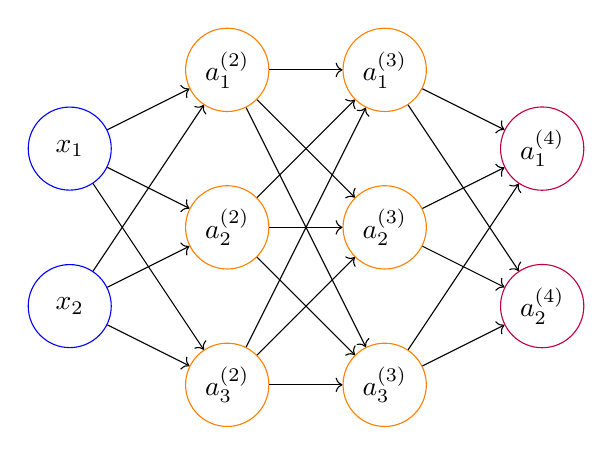
\begin{tikzpicture}
  \node[circle,
  minimum width =30pt ,
  minimum height =30pt ,draw=blue] (1) at(0,2){$x_1$};
  \node[circle,
  minimum width =30pt ,
  minimum height =30pt ,draw=blue] (2) at(0,0){$x_2$};
  \node[circle,
  minimum width =30pt ,
  minimum height =30pt ,draw=orange] (3) at(2,-1){$a_3^{(2)}$};
  \node[circle,
  minimum width =30pt ,
  minimum height =30pt ,draw=orange] (4) at(2,1){$a_2^{(2)}$};
  \node[circle,
  minimum width =30pt ,
  minimum height =30pt ,draw=orange] (5) at(2,3){$a_1^{(2)}$};
  \node[circle,
  minimum width =30pt ,
  minimum height =30pt ,draw=orange] (6) at(4,-1){$a_3^{(3)}$};
  \node[circle,
  minimum width =30pt ,
  minimum height =30pt ,draw=orange] (7) at(4,1){$a_2^{(3)}$};
  \node[circle,
  minimum width =30pt ,
  minimum height =30pt ,draw=orange] (8) at(4,3){$a_1^{(3)}$};
  \node[circle,
  minimum width =30pt ,
  minimum height =30pt ,draw=purple] (9) at(6,2){$a_1^{(4)}$};
  \node[circle,
  minimum width =30pt ,
  minimum height =30pt ,draw=purple] (10) at(6,0){$a_2^{(4)}$};
  \draw[->] (1) --(3);
  \draw[->] (1) --(4);
  \draw[->] (1) --(5);
  \draw[->] (2) --(3);
  \draw[->] (2) --(4);
  \draw[->] (2) --(5);
  \draw[->] (3) --(6);
  \draw[->] (3) --(7);
  \draw[->] (3) --(8);
  \draw[->] (4) --(6);
  \draw[->] (4) --(7);
  \draw[->] (4) --(8);
  \draw[->] (5) --(6);
  \draw[->] (5) --(7);
  \draw[->] (5) --(8);
  \draw[->] (6) --(9);
  \draw[->] (6) --(10);
  \draw[->] (7) --(9);
  \draw[->] (7) --(10);
  \draw[->] (8) --(9);
  \draw[->] (8) --(10);
  \end{tikzpicture}

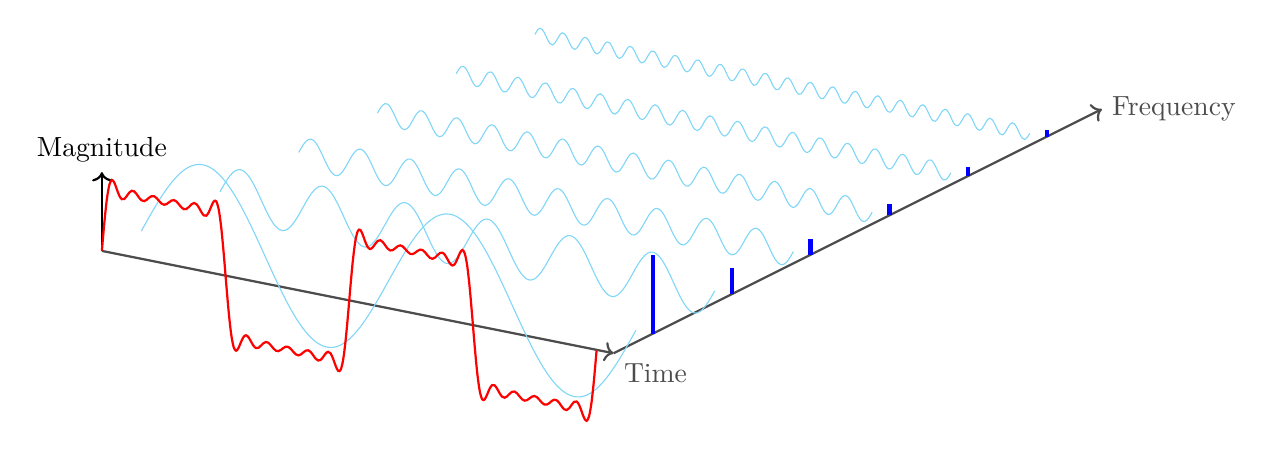
\begin{tikzpicture}[x={(1cm,0.5cm)},z={(0cm,0.5cm)},y={(1cm,-0.2cm)}]
  \draw[->,thick,black!70] (0,6.5,0) -- (6.2,6.5,0) node[right] {Frequency}; % 频率轴
  \draw[->,thick,black!70] (0,0,0) -- (0,6.5,0) node[below right] {Time}; % 时间轴
  \draw[->,thick] (0,0,0) -- (0,0,2) node[above] {Magnitude}; 
  
  \foreach \n in {0.5,1.5,...,5.5}{
  \draw [cyan!50, domain=0:2*pi,samples=200,smooth] 
   plot (\n,\x, {sin(4*\n*\x r)/\n });
  \draw[blue, ultra thick] (\n,6.5,0) -- (\n,6.5,1/\n);
  } % 频率逐渐增大振幅逐渐变小的正弦函数
  
  \draw [red, thick, domain=0:2*pi,samples=200,smooth] 
  plot (0,\x, {sin(4*0.5*\x r)/0.5 + sin(4*1.5*\x r)/1.5 + sin(4*2.5*\x r)/2.5 + sin(4*3.5*\x r)/3.5 + sin(4*4.5*\x r)/4.5 + sin(4*5.5*\x r)/5.5} ); 
  % 最后是手动加起来得到矩形波的逼近
\end{tikzpicture}

\blinddocument


\end{document}